\documentclass[review]{elsarticle}
\usepackage[T1]{fontenc}
\usepackage[ansinew]{inputenc}
\usepackage{amsmath}
\usepackage{amssymb}
\usepackage{tikz}
\usepackage{tikz-dimline}
\pgfplotsset{
  compat=1.5,
  legend image code/.code={
    \draw[mark repeat=2,mark phase=2]
    plot coordinates {
      (0cm,0cm)
      (0.15cm,0cm)        %% default is (0.3cm,0cm)
      (0.3cm,0cm)         %% default is (0.6cm,0cm)
    };
  }
}
\usepackage{xcolor}
\usepackage{pgfplots}
\usepackage{pgfplotstable}
\usepgfplotslibrary{groupplots,dateplot}
\usetikzlibrary{patterns,shapes.arrows,calc,external,decorations,shapes,positioning,arrows.meta}
\usepgfplotslibrary{colormaps}
\usetikzlibrary{pgfplots.colormaps}
\usepgfplotslibrary{fillbetween}
\tikzset{>=latex}
\pgfplotsset{compat=newest}

\begin{document}

    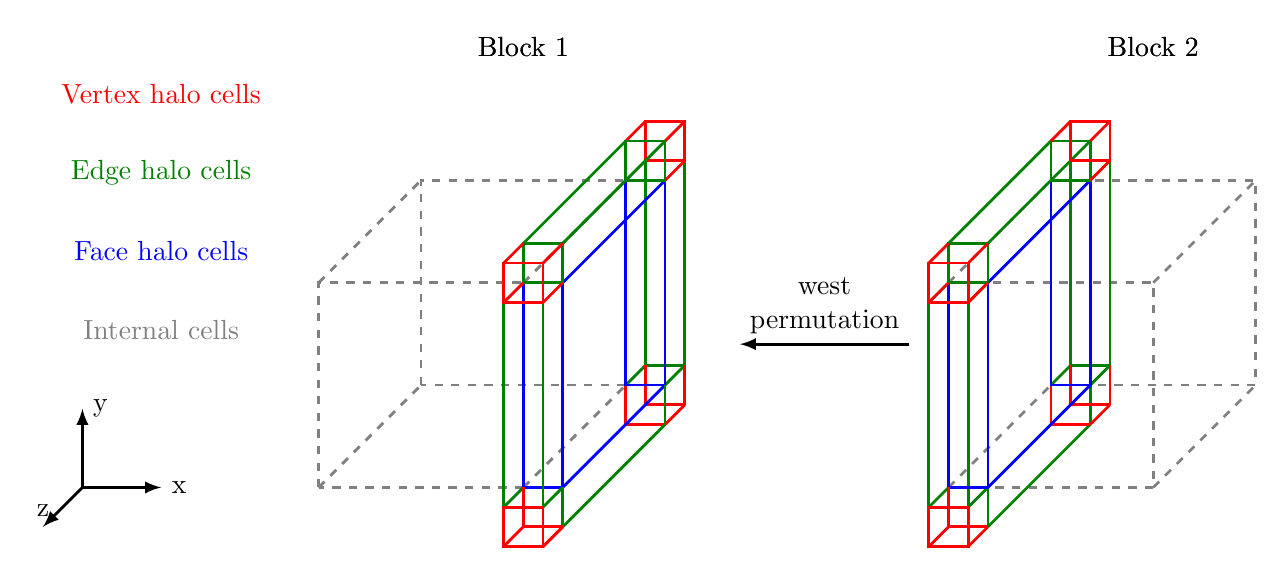
\begin{tikzpicture}

    % COORDINATE SYSTEM
    \draw[line width=1pt,->] (-3,0) -- (-2,0) node[right] {x};
    \draw[line width=1pt,->] (-3,0) -- (-3,1) node[right] {y};
    \draw[line width=1pt,->] (-3,0) -- (-3.5,-0.5) node[above] {z};

    \coordinate (O) at (0,0);
    \coordinate (L) at (2.6,2.6);
    \coordinate (HX) at (0.5,0);
    \coordinate (HY) at (0,0.5);
    \coordinate (VX) at ($0.5*(HX)$);
    \coordinate (VY) at ($0.5*(HY)$);

    % HALO NAMES
    \node[color=blue, align=right, color=black!50!white] at (-2,2) {Internal cells};
    \node[color=blue, align=right] at (-2,3) {Face halo cells};
    \node[color=green!50!black, align=right] at (-2,4) {Edge halo cells};
    \node[color=red!100!black, align=right] at (-2,5) {Vertex halo cells};

    % BLOCK 1
    \coordinate (L1) at ($0.5*(L)$);
    \coordinate (L2) at ($3*(L1)$);

    \draw[line width=1pt, dashed, color=black!50!white] (O) rectangle (L);
    \draw[line width=1pt, dashed, color=black!50!white] (L1) rectangle (L2);
    \draw[line width=1pt, dashed, color=black!50!white] (L) -- (L2);
    \draw[line width=1pt, dashed, color=black!50!white] (L|-O) -- (L2|-L1);
    \draw[line width=1pt, dashed, color=black!50!white] (O) -- (L1);
    \draw[line width=1pt, dashed, color=black!50!white] (L-|O) -- (L2-|L1);


    % BLOCK 1 EAST BOTTOM EDGE HALOS
    \coordinate (F1) at ($(HX)+(L)$);
    \coordinate (F2) at ($(HX)+(L2)$);
    \coordinate (E11) at ($(L2|-L1)+(VX)+(VY)$);
    \coordinate (E22) at ($(F2)+(VX)+(VY)$);
    \coordinate (E1) at ($(L)+(HX)+(HY)$);
    \coordinate (E2) at ($(L2)+(HX)+(HY)$);
    \draw[line width=1pt, color=green!50!black] (E11) rectangle (E22);
    \draw[line width=1pt, color=green!50!black] ($(L2|-L1)$) -- ($(L2|-L1)+(VX)+(VY)$);
    \draw[line width=1pt, color=green!50!black] ($(L2|-L1)+2*(VX)$) -- ($(L2|-L1)+3*(VX)+(VY)$);


    % BLOCK 1 EAST SOUTH BOTTOM VERTEX HALOS
    \coordinate (E1111) at ($(L2|-L1)+(HX)-(HY)$);
    \draw[line width=1pt, color=red!100!black] (E1111) -- ($(E1111)+(VX)+(VY)$);
    \draw[line width=1pt, color=red!100!black] (E1111) -- ($(E1111)-(HX)$);
    \draw[line width=1pt, color=red!100!black] ($(E1111)-(HX)$) -- ($(E1111)+(HY)-(HX)$);
    \draw[line width=1pt, color=red!100!black] ($(E1111)+(VX)+(VY)$) -- ($(E1111)+(VX)+(VY)+(HY)$);
    \draw[line width=1pt, color=red!100!black] ($(E1111)+(VX)+(VY)$) -- ($(E1111)-(VX)+(VY)$);
    \draw[line width=1pt, color=red!100!black] ($(E1111)-(VX)+(VY)$) -- ($(E1111)-(VX)+(VY)+(HY)$);


    % BLOCK 1 EAST FACE HALOS
    \coordinate (F1) at ($(HX)+(L)$);
    \coordinate (F2) at ($(HX)+(L2)$);
    \draw[line width=1pt, color=blue] (L|-O) rectangle (F1);
    \draw[line width=1pt, color=blue] (L2|-L1) rectangle (F2);
    \draw[line width=1pt, color=blue] (F1|-O) -- (F2|-L1);
    \draw[line width=1pt, color=blue] (F1|-L) -- (F2|-L2);

    % BLOCK 1 EAST TOP EDGE HALOS
    \coordinate (F1) at ($(HX)+(L)$);
    \coordinate (F2) at ($(HX)+(L2)$);
    \coordinate (E111) at ($(L|-O)-(VX)-(VY)$);
    \coordinate (E222) at ($(F1)-(VX)-(VY)$);
    \draw[line width=1pt, color=green!50!black] (E111) rectangle (E222);
    \draw[line width=1pt, color=green!50!black] (E111) -- (L|-O);
    \draw[line width=1pt, color=green!50!black] ($(E111)+(HX)$) -- ($(E111)+(HX)+(VX)+(VY)$);

    % BLOCK 1 EAST SOUTH EDGE HALOS
    \coordinate (F1) at ($(HX)+(L)$);
    \coordinate (F2) at ($(HX)+(L2)$);
    \coordinate (E111) at ($(L|-O)-(VX)-(VY)$);
    \coordinate (E222) at ($(F1)-(VX)-(VY)$);
    \draw[line width=1pt, color=green!50!black] ($(F1|-O)-(HY)$) -- ($(F2|-L1)-(HY)$);
    \draw[line width=1pt, color=green!50!black] ($(F1|-O)-(HY)$) -- ($(F1|-O)$);
    \draw[line width=1pt, color=green!50!black] ($(F2|-L1)-(HY)$) -- ($(F2|-L1)$);


    % BLOCK 1 EAST NORTH BOTTOM VERTEX HALOS
    \coordinate (V1) at ($(L2)+(VX)+(VY)$);
    \coordinate (V2) at ($(E2)+(VX)+(VY)$);
    \draw[line width=1pt, color=red!100!black] (V1) rectangle (V2);
    \draw[line width=1pt, color=red!100!black] (F2) -- (V2|-V1);
    \draw[line width=1pt, color=red!100!black] (E2) -- (V2);
    \draw[line width=1pt, color=red!100!black] (L2|-E2) -- (V1|-V2);


    % BLOCK 1 EAST NORTH EDGE HALOS
    \coordinate (E1) at ($(L)+(HX)+(HY)$);
    \coordinate (E2) at ($(L2)+(HX)+(HY)$);
    \draw[line width=1pt, color=green!50!black] (L) rectangle (E1);
    \draw[line width=1pt, color=green!50!black] (L2) rectangle (E2);
    \draw[line width=1pt, color=green!50!black] (E1) -- (E2);
    \draw[line width=1pt, color=green!50!black] (L|-E1) -- (L2|-E2);

    % BLOCK 1 EAST SOUTH TOP VERTEX HALOS
    \coordinate (V1) at ($(L2)+(VX)+(VY)$);
    \coordinate (V2) at ($(E2)+(VX)+(VY)$);
    \draw[line width=1pt, color=red!100!black] ($(E111)-(HY)$) rectangle ($(E111)+(HX)$);
    \draw[line width=1pt, color=red!100!black] ($(E111)-(HY)$) -- ($(E111)-(HY)+(VY)+(VX)$);
    \draw[line width=1pt, color=red!100!black] ($(E111)-(HY)+(HX)$) -- ($(E111)-(HY)+(VY)+(VX)+(HX)$);
    \draw[line width=1pt, color=red!100!black] ($(E111)-(HY)+(HX)$) -- ($(E111)-(HY)+(VY)+(VX)+(HX)$);
    \draw[line width=1pt, color=red!100!black] ($(L|-O)$) -- ($(L|-O)-(HY)$);
    \draw[line width=1pt, color=red!100!black] ($(L|-O)-(HY)$) -- ($(L|-O)-(HY)+(HX)$);

    % BLOCK 1 EAST NORTH TOP VERTEX HALOS
    \coordinate (V1) at ($(L2)+(VX)+(VY)$);
    \coordinate (V2) at ($(E2)+(VX)+(VY)$);
    \draw[line width=1pt, color=red!100!black] ($(L)-(VX)-(VY)$) rectangle ($(L)+(VX)+(VY)$);
    \draw[line width=1pt, color=red!100!black] ($(L)$) -- ($(L)-(VX)-(VY)$);
    \draw[line width=1pt, color=red!100!black] ($(L)+(VX)-(VY)$) -- ($(L)+(HX)$);
    \draw[line width=1pt, color=red!100!black] ($(L)+(VX)+(VY)$) -- ($(L)+(HX)+(HY)$);
    \draw[line width=1pt, color=red!100!black] ($(L)-(VX)+(VY)$) -- ($(L)+(HY)$);



    % BLOCK 2
    \coordinate (OFFSETX) at (8,0);
    \coordinate (OO) at ($(O)+(OFFSETX)$); % (10,0)
    \coordinate (LL) at ($(L)+(OFFSETX)$); % (14,4)
    \coordinate (LL1) at ($(LL)-(L1)$); % (12,2)
    \coordinate (LL2) at ($(LL1)+(L)$);

    \draw[line width=1pt, dashed, color=black!50!white] (OO) rectangle (LL);
    \draw[line width=1pt, dashed, color=black!50!white] (LL1) rectangle (LL2);
    \draw[line width=1pt, dashed, color=black!50!white] (LL) -- (LL2);
    \draw[line width=1pt, dashed, color=black!50!white] (LL|-OO) -- (LL2|-LL1);
    \draw[line width=1pt, dashed, color=black!50!white] (OO) -- (LL1);
    \draw[line width=1pt, dashed, color=black!50!white] (LL-|OO) -- (LL2-|LL1);

    % BLOCK 2 NORTH FACE HALOS
    \coordinate (FF1) at ($(LL)+(HY)$);
    \coordinate (FF2) at ($(LL2)-(L|-HX)$);
    \coordinate (FF3) at ($(LL2)+(HY)$);
    \coordinate (FF4) at ($(OO|-L)+(HY)$);
    \coordinate (FF5) at ($(FF2)+(HY)$);

    % BLOCK 2 WEST BOTTOM EDGE HALOS
    \coordinate (FFF1) at ($(OO|-L)+(HX)$);
    \coordinate (FFF2) at ($(LL1|-LL2)+(HX)$);
    \coordinate (FFF3) at ($(OO)+(HX)$);
    \coordinate (FFF4) at ($(LL1)+(HX)$);
    \draw[line width=1pt, color=green!50!black] ($(LL1)+(VY)+(VX)$) rectangle ($(FFF2)+(VY)+(VX)$);
    \draw[line width=1pt, color=green!50!black] ($(LL1)+(VY)+(VX)$) -- ($(LL1)$);
    \draw[line width=1pt, color=green!50!black] ($(LL1)+(HX)$) -- ($(LL1)+(HX)+(VX)+(VY)$);

    % BLOCK 2 WEST TOP EDGE HALOS
    \draw[line width=1pt, color=green!50!black] ($(OO)-(VY)-(VX)$) rectangle ($(FFF1)-(VY)-(VX)$);
    \draw[line width=1pt, color=green!50!black] ($(FFF1)-(VY)-(VX)$) -- ($(FFF1)$);
    \draw[line width=1pt, color=green!50!black] ($(FFF1)-(VY)-(VX)-(HX)$) -- ($(FFF1)-(HX)$);
    \draw[line width=1pt, color=green!50!black] ($(OO)-(VY)-(VX)$) -- ($(OO)$);
    \draw[line width=1pt, color=green!50!black] ($(OO)-(VY)+(VX)$) -- ($(OO)+(HX)$);

    % BLOCK 2 WEST TOP EDGE HALOS
    \draw[line width=1pt, color=green!50!black] ($(FFF3)-(HY)$) -- ($(FFF4)-(HY)$);
    \draw[line width=1pt, color=green!50!black] ($(FFF4)-(HY)$) -- ($(FFF4)$);
    \draw[line width=1pt, color=green!50!black] ($(FFF3)-(HY)$) -- ($(FFF3)$);
    \draw[line width=1pt, color=green!50!black] ($(FFF3)-(HY)$) -- ($(FFF3)-(HY)-(HX)$);
    \draw[line width=1pt, color=green!50!black] ($(FFF4)-(HY)$) -- ($(FFF4)-(HY)-(HX)$);
    \draw[line width=1pt, color=green!50!black] ($(FFF4)-(HY)-(HX)$) -- ($(FFF4)-(HX)$);

    % BLOCK 2 WEST NORTH TOP VERTEX HALOS
    \draw[line width=1pt, color=red!100!black] ($(LL1)+(HX)-(HY)$) -- ($(LL1)+(HX)-(HY)+(VY)+(VX)$);
    \draw[line width=1pt, color=red!100!black] ($(LL1)$) -- ($(LL1)-(HY)$);
    \draw[line width=1pt, color=red!100!black] ($(LL1)-(HY)$) -- ($(LL1)-(HY)+(HX)$);
    \draw[line width=1pt, color=red!100!black] ($(LL1)+(HX)-(VY)+(VX)$) -- ($(LL1)+(HX)-(VY)+(VX)+(HY)$);
    \draw[line width=1pt, color=red!100!black] ($(LL1)+(HX)-(VY)+(VX)$) -- ($(LL1)+(HX)-(VY)+(VX)-(HX)$);
    \draw[line width=1pt, color=red!100!black] ($(LL1)+(HX)-(VY)+(VX)-(HX)$) -- ($(LL1)+(HX)-(VY)+(VX)-(HX)+(HY)$);

    % BLOCK 2 WEST FACE HALOS
    \coordinate (FFF1) at ($(OO|-L)+(HX)$);
    \coordinate (FFF2) at ($(LL1|-LL2)+(HX)$);
    \coordinate (FFF3) at ($(OO)+(HX)$);
    \coordinate (FFF4) at ($(LL1)+(HX)$);
    \draw[line width=1pt, color=blue] (OO) rectangle (FFF1);
    \draw[line width=1pt, color=blue] (LL1) rectangle (FFF2);
    \draw[line width=1pt, color=blue] (FFF3) -- (FFF4);
    \draw[line width=1pt, color=blue] (FFF1) -- (FFF2);

    % BLOCK 2 SEND EDGE HALOS
    \coordinate (EEE1) at ($(OO|-L)+(HX)+(HY)$);
    \coordinate (EEE2) at ($(LL1|-LL2)+(HX)+(HY)$);
    \coordinate (EEE3) at ($(OO|-LL)+(HY)$);
    \coordinate (EEE4) at ($(LL1|-LL2)+(HY)$);
    \draw[line width=1pt, color=green!50!black] (OO|-LL) rectangle (EEE1);
    \draw[line width=1pt, color=green!50!black] (LL1|-LL2) rectangle (EEE2);
    \draw[line width=1pt, color=green!50!black] (EEE1) -- (EEE2);
    \draw[line width=1pt, color=green!50!black] (EEE3) -- (EEE4);

    % BLOCK 2 NORTH BOTTOM EDGE HALOS
    \coordinate (VV1) at ($(FF2)-(HX)$);
    \coordinate (VV2) at ($(VV1)+(VX)+(VY)$);
    \coordinate (VV3) at ($(VV1)+(HY)$);
    \coordinate (VV4) at ($(VV2)+(HY)$);

    % BLOCK 2 SEND VERTEX HALOS
    \coordinate (VVV1) at ($(LL1|-LL2)+(VX)+(VY)$);
    \coordinate (VVV2) at ($(VVV1)+(HY)+(HX)$);
    \coordinate (VVV3) at ($(LL1|-LL2)+(HX)$);
    \coordinate (VVV4) at ($(VVV1)+(HX)$);
    \coordinate (VVV5) at ($(LL1|-LL2)+(HY)$);
    \coordinate (VVV6) at ($(VVV1)+(HY)$);
    \draw[line width=1pt, color=red!100!black] (VVV1) rectangle (VVV2);
    \draw[line width=1pt, color=red!100!black] (EEE2) -- (VVV2);
    \draw[line width=1pt, color=red!100!black] (VVV3) -- (VVV4);
    \draw[line width=1pt, color=red!100!black] (VVV5) -- (VVV6);

    % BLOCK 2 WEST SOUTH TOP VERTEX HALOS
    \draw[line width=1pt, color=red!100!black] ($(OO)-(VX)-(VY)-(HY)$) rectangle ($(OO)-(VY)+(VX)$);
    \draw[line width=1pt, color=red!100!black] ($(OO)-(VX)-(VY)-(HY)$) -- ($(OO)-(HY)$);
    \draw[line width=1pt, color=red!100!black] ($(OO)+(VX)-(VY)-(HY)$) -- ($(OO)+(HX)-(HY)$);
    \draw[line width=1pt, color=red!100!black] ($(OO)$) -- ($(OO)-(HY)$);
    \draw[line width=1pt, color=red!100!black] ($(OO)-(HY)+(HX)$) -- ($(OO)-(HY)$);

    % BLOCK 2 WEST NORTH TOP VERTEX HALOS
    \draw[line width=1pt, color=red!100!black] ($(OO|-LL)-(VX)-(VY)$) rectangle ($(OO|-LL)+(VY)+(VX)$);
    \draw[line width=1pt, color=red!100!black] ($(OO|-LL)-(VX)-(VY)$) -- ($(OO|-LL)$);
    \draw[line width=1pt, color=red!100!black] ($(OO|-LL)-(VX)-(VY)+(HY)$) -- ($(OO|-LL)+(HY)$);
    \draw[line width=1pt, color=red!100!black] ($(OO|-LL)+(VX)-(VY)+(HY)$) -- ($(OO|-LL)+(HY)+(HX)$);
    \draw[line width=1pt, color=red!100!black] ($(OO|-LL)+(VX)-(VY)$) -- ($(OO|-LL)+(HX)$);

    % COMMS
    \coordinate (COMMS1) at ($(OO)+0.8*(HY|-L)-5.3*(HX)$);
    \coordinate (COMMS2) at ($(OO)+0.8*(HY|-L)-1*(HX)$);

    \coordinate (COMMS3) at ($(OO)+0.7*(HY|-L)-5.3*(HX)$);
    \coordinate (COMMS4) at ($(OO)+0.7*(HY|-L)-1*(HX)$);
    \draw[line width=1pt,<-] (COMMS3) -- (COMMS4) node[midway, above, align=center] {west \\ permutation};

    % BLOCK NAMES
    \node at ($(L) + 6*(HY)$) {Block 1};
    \node at ($(LL) + 6*(HY)$) {Block 2};

    \node at ($(L) + 6*(HY)$) {Block 1};
    \node at ($(LL) + 6*(HY)$) {Block 2};


\end{tikzpicture}

\end{document}